% !TEX root = ../Asymptotic-CBP.tex

\section{Proofs for Section~\ref{sec-contbp-thin}}

%%%%%%%%%%%%%%%%%%%%%%%%%%%%%%%%%%%%%%%%%%%
\subsection{Proof of Proposition~\ref{prop-cbp-gammaconv}}
\label{prop-cbp-gammaconv-proof}


% \begin{proof}
We observe that our embedding of the discrete problem into the continuous one, that is $\mn=\sum_{i=0}^{\taillegridn-1} \veccont^{(n)}_{i} \delta_{i\stepsizen+\shiftcont_i/\veccont_i }$, yields $\|\veccont^{(n)}\|_1=\abs{\mn}(\TT)={\mn}(\TT)$.
For the liminf inequality, let $(\mn)_{n\in\NN}$ be of the form~\eqref{eq-cbp-measure} which weakly* converges towards $m$. We notice that $\Phi'_{\Gg_n}\shiftcont^{(n)}= \Phi' (\sum_{i=0}^{\taillegridn-1}\shiftcont^{(n)}_i\delta_{i\stepsizen})$, where $\Phi':m\mapsto \int_\TT \varphi'(x)\d m(x)$ is continuous from $\Mm(\TT)$ to $\Hh$ (in the strong topologies). Moreover,
\begin{align*}
  \left|\sum_{i=0}^{\taillegridn-1}\shiftcont^{(n)}_i\delta_{i\stepsizen}\right|(\TT) &\leq \frac{\stepsizen}{2}\left(\sum_{i=0}^{\taillegridn-1}\veccont^{(n)}_i\right)  
    \leq \frac{\stepsizen}{2\la}\left(\frac{1}{2}\normH{y}^2+1\right)\to 0,
%    \stackrel{*}{\rightharpoonup} 0,
  \end{align*}
  so that $\Phi'_{\Gg_n}\shiftcont^{(n)}$ converges strongly towards $0$ in $\Hh$.
Additionally, $\Phi_{\Gg_n}\veccont^{(n)}= \Phi (\sum_{i=0}^{\taillegridn-1}\veccont^{(n)}_i\delta_{i\stepsizen})$ and for all $\psi\in \Cont(\TT)$, 
  \begin{align*}
    \left|\left\langle\sum_{i=0}^{\taillegridn-1} \veccont_{i}^{(n)} \delta_{i\stepsizen+\shiftcont_i/\veccont_i }- \sum_{i=0}^{\taillegridn-1} \veccont_{i}^{(n)} \delta_{i\stepsizen}, \psi \right\rangle\right| &= \left|\sum_{i=0}^{\taillegridn-1} \veccont_{i}^{(n)} (\psi(i\stepsizen+\shiftcont_i/\veccont_i)-\psi(i\stepsizen))\right|\\
    &\leq \sum_{i=0}^{\taillegridn-1} \veccont_{i}^{(n)} \omega_\psi\left(\frac{\stepsizen}{2} \right) \to 0
  \end{align*}
  where $\omega_\psi: t\mapsto \sup_{|x'-x|\leq t}|\psi(x)-\psi(x')|$ is the modulus of continuity of $\psi$. As a result, $\sum_{i=0}^{\taillegridn-1} \veccont_{i}^{(n)} \delta_{i\stepsizen}-\mn \stackrel{*}{\rightharpoonup} 0$ so that $\sum_{i=0}^{\taillegridn-1} \veccont_{i}^{(n)} \delta_{i\stepsizen}$ weakly* converges to $m$. Hence, $\Phi_{\Gg_n}\veccont^{(n)}$ weakly converges towards $\Phi m$ in $\Hh$.
To sum up, $\Phi_{\Gg_n}\veccont^{(n)}+\Phi'_{\Gg_n}\shiftcont^{(n)}-y$ weakly converges towards $\Phi m-y$ and we conclude by invoking the lower semi-continuity of both terms:
      \begin{align*}
        \liminf_{n\to +\infty}\left(\la \|\veccont^{(n)}\|_1+\frac{1}{2}\normH{\Phi_{\Gg_n}\veccont^{(n)}+\Phi'_{\Gg_n}\shiftcont^{(n)}-y}^2\right) &\geq \liminf_{n\to +\infty}\left(\la \abs{\mn}(\TT) + \frac{1}{2}\normH{\Phi_{\Gg_n}\veccont^{(n)}+\Phi'_{\Gg_n}\shiftcont^{(n)}-y}^2\right)\\
        &\geq \la m(\TT) + \frac{1}{2}\normH{\Phi m-y}^2.
      \end{align*}
 
      For the limsup inequality, we build a recovery sequence $\mn$ by choosing $\veccont^{(n)}_k=m([k\stepsizen,(k+1)\stepsizen))$ and $\shiftcont^{(n)}_k=0$ for all $k\in \seg{0}{\taillegridn-1}$. Then, for all $n$, $\|\veccont^{(n)}\|_1=m(\TT)$ and 
        \begin{align*}
          \normH{\Phi\left(\sum_{i=0}^{\taillegridn-1} \veccont_{i}^{(n)} \delta_{i\stepsizen}\right) -\Phi m}&\leq \sum_{i=0}^{\taillegridn-1}\normH{\int_{[i\stepsizen,(i+1)\stepsizen)}(\varphi(t)-\varphi(i\stepsizen))\d m(t)}\\
                                                                                                             &\leq m(\TT)\omega_\phi\left(\stepsizen \right)\to 0
        \end{align*}
since $\varphi$ is uniformly continuous on $\TT$. As a result, $\Phi \mn-y$ strongly converges towards $\Phi m-y$ and the limsup inequality is proved.
  % \end{proof}




%%%%%%%%%%%%%%%%%%%%%%%%%%%%%%%%%%%%%%%%%%%%%%%%%%%%%%
  \section{Proofs of Section~\ref{sec-asympt-support}}
  \label{sec-apx-asympt-support}
  The following lemma is central in our analysis. It studies sequences of dual certificates $(\mun)_{n\in\NN}$. For $0<r<\frac{1}{2} \min_{\nu\neq \nu'} |x_\nu - x_{\nu'}|$, $\nu\in\{1,\ldots,N\}$, it will be useful to consider the sets:
\begin{align*}
  \Sright(r)\eqdef\enscond{t\in \Gg_n\cap(x_\nu-r,x_\nu+r)}{\left(\mun+\frac{\stepsizen}{2}{\mun}'\right)(t)=1},\\
  \Sleft(r)\eqdef\enscond{t\in \Gg_n\cap(x_\nu-r,x_\nu+r)}{\left(\mun-\frac{\stepsizen}{2}{\mun}'\right)(t)=1}.
\end{align*}



\begin{lem}
  Let $(x_1,\ldots, x_N)\in \TT^N$ pairwise distinct, and let $\{\mun\}_{n\in\NN}\in (\Cont^3(\TT))^\NN$ be a sequence of functions which converges uniformly towards some $\mui$ (and similarly for the derivatives) such that for all $\nu\in\{1,\ldots, N\}$, $\mui(x_\nu)=1$ and for all $t\in \TT\setminus\{x_1,\ldots,x_N\}$, $\mui(t)<1$.

\begin{enumerate}
  \item Then 
\begin{align}
  \limsup_{n\to +\infty} \enscond{t\in \Gg_n}{\mun(t)+\frac{\stepsizen}{2}|{\mun}'(t)|=1}\subset \{x_1,\ldots, x_N\}.\label{eq-cbp-limsup}
\end{align} In particular for $r>0$ small enough,
there exists $n_0\in\NN$ such that for $n\geq n_0$
 \begin{align*}
   \enscond{t\in \Gg_n}{\mun(t)+\frac{\stepsizen}{2}|{\mun}'(t)|=1} = \bigcup_{\nu=1}^N  \left(\Sright(r)\cup  \Sleft(r)\right) \subset \bigcup_{\nu=1}^N(x_\nu-r,x_\nu+r).
 \end{align*}
\end{enumerate}
Assume moreover that for all $n\in\NN$ and all $t\in\Gg_n$, $\mun(t)+\frac{\stepsizen}{2}|{\mun}'(t)| \leq 1$. For each $\nu \in\{1,\ldots,N\}$:
\begin{enumerate}
\setcounter{enumi}{1}
\item\label{item-deriv2} If $\mui''(x_\nu)\neq 0$, then there exists $n_0\in\NN$ such that for $n\geq n_0$, each set $\Sright(r)$ and $\Sleft(r)$ is of the form
$\emptyset$, $\{i\stepsizen\}$, or $\{i\stepsizen,(i+1)\stepsizen\}$, and if both sets are nonempty:
\begin{align*}
  \max \Sright(r) \leq \min \Sleft(r).
\end{align*}

\item If $\mui^{(3)}(x_\nu)\neq 0$, then there exists $n_0\in\NN$ such that for each $n\geq n_0$, $\Sright(r)=\emptyset$ or $\Sleft(r)=\emptyset$.
\item\label{item-deriv4} If $\mui^{(4)}(x_\nu)\neq 0$, the set of $n\in\NN$ such that $\Sright(r)=\{(i_n-1)\stepsizen,i_n\stepsizen\}$ and $\Sleft (r)= \{i_n\stepsizen,(i_n+1)\stepsizen\}$ (with the same $i_n\in\seg{0}{\taillegridn-1}$) is finite.
\end{enumerate}
\label{lem-cbp-dualspikes}
\end{lem}

\begin{proof}
%   Observe that both $\mu^{n} + \frac{\stepsizen}{2}{\mu^{n}}'$ and $\mu^{n} - \frac{\stepsizen}{2}{\mu^{n}}'$ converge uniformly towards $\mu^{\infty}$ as $n\to +\infty$ (and similarly for the derivatives).
   \begin{enumerate}
     \item  For all $\tilde{r}\in(0,r)$, by compactness, $\sup \enscond{\mui(t) }{t\in\TT\setminus\bigcup (x_\nu-\tilde{r},x_\nu+\tilde{r})}<1$. Thus by uniform convergence there exists  $n_0\in \NN$ such that for all $n\geq n_0$, $(\mun \pm \frac{\stepsizen}{2}{\mun}')<1$ on $\TT\setminus\bigcup_{\nu=1}^N (x_\nu-\tilde{r},x_\nu+\tilde{r})$, and the first claim is proved.

   \item If moreover $\mui''(x_\nu)\neq 0$, it is in fact negative. Choosing $\tilde{r}\in(0,r)$ small enough and then $n$ large enough, we may assume that ${\mun}'' <-k_0$ in $(x_\nu-\tilde{r},x_\nu+\tilde{r})$, for some $k_0>0$, and by~\eqref{eq-cbp-limsup} that $\Sright(r)\cup\Sleft(r)\subset (x_{\nu}-\tilde{r},x_{\nu}+\tilde{r})$. By uniform convergence, ${\mun}''+\frac{\stepsizen}{2}|\mun^{(3)}|<-\frac{k_0}{2}$ for $n$ large enough, so that both functions $\mun + \frac{\stepsizen}{2}{\mun}'$ and $\mun - \frac{\stepsizen}{2}{\mun}'$ are strictly concave in $(x_\nu-\tilde{r},x_\nu+\tilde{r})$. This implies that $\Sright(r)$ (resp. $\Sleft(r)$) is of the form $\emptyset$, $\{i\stepsizen\}$, or $\{i\stepsizen,(i+1)\stepsizen\}$.

     Observe also that $\mun + \frac{\stepsizen}{2}{\mun}' -(\mun - \frac{\stepsizen}{2}{\mun}')= \stepsizen{\mun}'$.
     Since the function ${\mun}'$ is strictly decreasing in $(x_\nu-\tilde{r},x_\nu+\tilde{r})$, it vanishes at most once. If $\Sright(r)\neq\emptyset$ and $\Sleft(r)\neq\emptyset$, it must change sign in $(x_\nu-\tilde{r},x_\nu+\tilde{r})$ and thus it vanishes exactly once, at some $\xi\in (x_\nu-\tilde{r},x_\nu+\tilde{r})$. 
Then for $t\in (x_\nu-\tilde{r},\xi)$, 
\begin{align*}
  (\mun - \frac{\stepsizen}{2}{\mun}')(t)=(\mun + \frac{\stepsizen}{2}{\mun}')(t)- \stepsizen \mun'(t)\leq 1 - \stepsizen \mun'(t)<1
\end{align*}
so that $\min \Sleft(r)\geq\xi$. Similarly $\max \Sright(r)\leq \xi$.

\item By contradiction, assume that the set of $n'\in\NN$ such that $\Srightp(r)\neq \emptyset$ and $\Sleftp(r)\neq \emptyset$ is infinite. We may extract a subsequence $n=n'(m)$ such that there exists $i_n,j_n\in\seg{0}{\taillegridn-1}$ (denoted hereafter $i,j$) with $i\stepsizen\in \Sright(r_m)$, $j\stepsizen\in \Sleft$.
 Combining the Taylor expansions of $\mun$ and $({\mun})'$ around $i\stepsizen$ (resp. $j\stepsizen$), we get
\begin{align*}
  1&\geq \mun((i+1)\stepsizen)-\frac{\stepsizen}{2}{\mun}'((i+1)\stepsizen)\\
   & =  \underbrace{\mun(i\stepsizen) +\stepsizen{\mun}'(i\stepsizen)(1-\frac{1}{2} )}_{=1} +\stepsizen^2{\mun}''(i\stepsizen)\underbrace{\left(\frac{1}{2!} -\frac{1}{2}\right)}_{=0} + \stepsizen^3 {\mun}^{(3)}(i\stepsizen)\al_3\\
   & \qquad\qquad+ \stepsizen^4\int_0^1 {\mun}^{(4)}(i\stepsizen+t\stepsizen)\left(\frac{(1-t)^3}{3!} -\frac{(1-t)^2}{2!\times 2}\right)\d t, \mbox{ and }\\
  1&\geq \mun((j-1)\stepsizen)+\frac{\stepsizen}{2}{\mun}'((j-1)\stepsizen)\\
   & =  \underbrace{\mun(j\stepsizen) -\stepsizen{\mun}'(j\stepsizen)(1-\frac{1}{2} )}_{=1} +\stepsizen^2{\mun}''(j\stepsizen)\underbrace{\left(\frac{1}{2!} -\frac{1}{2}\right)}_{=0} -\stepsizen^3 {\mun}^{(3)}(j\stepsizen)\al_3\\
   & \qquad\qquad+ \stepsizen^4\int_0^1 {\mun}^{(4)}(j\stepsizen-t\stepsizen)\left(\frac{(1-t)^3}{3!} -\frac{(1-t)^2}{2!\times 2}\right)\d t
\end{align*}
where $\al_k$ is defined in~\eqref{eq?defn-alphak}.
Now, let $n\to +\infty$. By~\eqref{eq-cbp-limsup}, $i\stepsizen\to x_{\nu}$ and $j\stepsizen\to x_\nu$, and using the uniform convergence of $\mun^{(k)}$ towards $\mui^{(k)}$, dividing by $\stepsizen^3$, we obtain respectively $0\geq -\mui^{(3)}(x_\nu)\times\frac{1}{12}$ and $0\geq \mui^{(3)}(x_\nu)\times \frac{1}{12}$, thus $\mui^{(3)}(x_\nu)=0$.

\item Assume, by contradiction, that the mentioned set is infinite. For such $n$, a Taylor expansion at $i\stepsizen$ yields (we write $i$ for $i_n$):
\begin{align*}
  1&=\mun((i+1)\stepsizen)-\frac{\stepsizen}{2}{\mun}'((i+1)\stepsizen)\\
   & =  \underbrace{\mun(i\stepsizen) +\frac{\stepsizen}{2}{\mun}'(i\stepsizen)}_{=1} + \gamma_3\stepsizen^3 {\mun}^{(3)}(i\stepsizen)+ \gamma_4\stepsizen^4 {\mun}^{(4)}(i\stepsizen)\\
   &\quad\quad+\stepsizen^5\int_0^1 {\mun}^{(5)}(i\stepsizen+t\stepsizen)\left(\frac{(1-t)^4}{4!} -\frac{(1-t)^3}{3!\times 2}\right)\d t, \mbox{ and }\\
  1&= \mun((i-1)\stepsizen)+\frac{\stepsizen}{2}{\mun}'((i-1)\stepsizen)\\
   & =  \underbrace{\mun(i\stepsizen) -\frac{\stepsizen}{2}{\mun}'(i\stepsizen)}_{=1} - \gamma_3\stepsizen^3 {\mun}^{(3)}(i\stepsizen)+ \gamma_4\stepsizen^4 {\mun}^{(4)}(i\stepsizen)\\
   &\quad \quad+  \stepsizen^5\int_0^1 {\mun}^{(5)}(i\stepsizen+t\stepsizen)\left(\frac{(1-t)^4}{4!} -\frac{(1-t)^3}{3!\times 2}\right)\d t,
\end{align*}
with $\gamma_k=\frac{1}{k!}- \frac{1}{(k-1)!\times 2}$. Summing both equalities, dividing by $\stepsizen^4$ and taking the limit $n\to+\infty$ yields $(\mui)^{(4)}(x_\nu)=0$, a contradiction.
   \end{enumerate}
\end{proof}

This other lemma focusses on the limit of the sets $D^n$ defined in~\eqref{eq-defn-Dn}.

\begin{lem}
As $n\to+\infty$, the sets $D^n$ converge towards $D^\infty$ defined in~\eqref{eq-defn-Dinf} (in the sense of set convergence).
\label{lem-cbp-cvset}
\end{lem}
\begin{proof}
  We observe that $E^n \subset D^n\subset F^n$, where
  \begin{align*}
    E^n&\eqdef \enscond{p\in \Hh}{\max_{t\in \TT}(\Phi^*p)(t)+\frac{\stepsizen}{2}|(\Phi^*p)'(t)| \leq 1},\\
    F^n&\eqdef \enscond{p\in \Hh}{\max_{k\in\seg{0}{\taillegridn-1}}\Phi^*p(k\stepsizen)\leq 1}
  \end{align*}
so that it suffices to prove that $E^n$ and $F^n$ converge towards $D^\infty$. 
On the one hand, it is clear that $D^\infty=\bigcap_{n\in\NN} F^n$, and the sequence $F^n$ is non-increasing.
On the other hand, it is possible to check that $D^\infty=\overline{\bigcup_{n\in \NN}E^{n}}$, and the sequence $E^n$ is non-decreasing.
As a consequence, the claimed set convergences hold  (see~\cite[Ex. 4.3]{rockafellarwets}).
\end{proof}

Let us recall that the dual problem to~\eqref{eq-thin-cbpasso} is the projection onto the closed convex set
\begin{align*}
  D^n &\eqdef\enscond{p\in \Hh}{(\Phi^* p)(i\stepsizen) + \frac{\stepsizen}{2}|(\Phi^*p)'(i\stepsizen)|\leq 1}.
\end{align*}

Since the set convergence of $D^n$ (see Lemma~\ref{lem-cbp-cvset} above) implies the convergence of the projections onto~$D^n$ (see~\cite{rockafellarwets}, or~\cite{2013-duval-sparsespikes} for a direct proof in a similar context), we obtain:

\begin{lem}\label{prop-cbp-cvdual}
  Let $p_{\la,n}$ (resp. $p_{\la,\infty}$) be a solution of~\eqref{eq-thin-dual-cbpasso} (resp.~\eqref{eq-beurl-dual-cbpasso}), and $\muln=\Phi^*p_{\la,n}$ (resp. $\muli=\Phi^*p_{\la,\infty}$). Then 
  \begin{align*}
    \lim_{n\to +\infty} p_{\la,{n}} &=p_{\la,\infty} \mbox{ strongly in $\Hh$,}\\ 
    \lim_{n\to +\infty} \muln^{(k)} &=\muli^{(k)} \mbox{ in the sense of the uniform convergence, for all $k\in \NN$ up to the regularity of $\varphi$.} 
\end{align*}
\end{lem}

We are now in position to prove Proposition~\ref{prop-cbp-thin-supplambda}.

\begin{proof}[Proof of Proposition~\ref{prop-cbp-thin-supplambda}]
  By Lemma~\ref{prop-cbp-cvdual}, we know that the dual certificates $\muln$ converge towards $\muli$. By Lemma~\ref{lem-cbp-dualspikes} (i) and the optimality conditions, we have thus $\limsup_{n\to+\infty} (\supp(\mln))\subset \{x_1,\ldots,x_N\}$.
  
  If $\mli$ is the unique solution, assume by contradiction that $\liminf (\supp (\mln))\subsetneq \{x_1,\ldots,x_N\}$. Then there is some $\nu$, some $\varepsilon>0$ such that (up to a subsequence) $(\supp(\mln))\cap (x_\nu-\varepsilon,x_\nu+\varepsilon)=\emptyset$. This contradicts the $\Gamma$-convergence result (Prop.~\ref{prop-cbpthin-convergence}) which ensures that $\mln$ converges towards $\mli$ in the weak* topology. As a result $\lim_{n\to+\infty} (\supp (\mln))=\{x_1,\ldots,x_N\}$.

  If $\mu_{\la,\infty}''(x_\nu)\neq 0$, Lemma~\ref{lem-cbp-dualspikes} ensures that the sets $\Sright(r)$ and $\Sleft(r)$ are of the form $\emptyset$, $\{i\stepsizen\}$, or $\{i\stepsizen,(i+1)\stepsizen\}$. Moreover, since $\lim_{n\to+\infty} (\supp \mln)=\{x_1,\ldots,x_N\}$ we must have $\Sright(r)\neq \emptyset$ or $\Sleft(r)\neq \emptyset$. Using the fact that $\max \Sright(r)  \leq \min \Sleft(r)$, one may check that the only possible saturation points of $\muln+\frac{\stepsizen}{2}\muln'$ and  $\muln-\frac{\stepsizen}{2}{\muln}'$ are given in Table~\ref{tab-nbdirac}. The optimality conditions of Proposition~\ref{prop-optim-cbp} imply that $\mln$ is at most a sum of Dirac masses at those locations.

  If $\muli^{(3)}(x_\nu)\neq 0$, Lemma~\ref{lem-cbp-dualspikes} (iii) implies that for $n$ large enough, $\Sright(r)=\emptyset$ or $\Sright(r)=\emptyset$ (but not both). Hence there are at most two (successive) saturations, produced either by $\muln+\frac{\stepsizen}{2} \muln'$ or by $\muln-\frac{\stepsizen}{2}\muln'$.
\end{proof}



%%%%%%%%%%%%%%%%%%%%%%%%%%%%%%%%%%%%%%%%%%%
\subsection{Sufficient Condition for Asymptotic Solutions}
\label{sec-asymp-sol}

The following property ensures that $m_0$ is a solution to~\eqref{eq-thin-cbp} for each $n$ large enough.

\begin{lem}
  Assume that there exists a function $\muc\in \Im \Phi^*$, such that for all $t\in\TT\setminus \{x_{0,1},\ldots ,x_{0,N} \}$, $\muc(t)<1$ and 
\begin{align*}
  \forall \nu\in \{1,\ldots, N\}, \ \muc(x_{0,\nu})=1, \ \muc''(x_{0,\nu})\neq 0, \ \muc^{(3)}(x_{0,\nu})=0,\ \muc^{(4)}(x_{0,\nu})>0.
\end{align*}
Then, for all $n$ large enough, $\muc$ is a dual certificate for $m_0= \sum_{\nu=1}^N \alpha_{0,\nu}\delta_{x_{0,\nu}}$ for~\eqref{eq-thin-cbp}, and $m_0$ is a solution to~\eqref{eq-thin-cbp}. Moreover, if $\Gamma_{x_0}$ has full rank, this solution is unique.
%of REF satisify $(i-\frac{1}{2})\De< i\De + \tau_i<(i+\frac{1}{2})$
\label{lem-source-cbp}
\end{lem}

\begin{rem} The condition $\muc^{(3)}(x_{0,\nu})=0$ is natural since our aim is to build a certificate which is valid for all $n$, hence Lemma~\ref{lem-cbp-dualspikes} applies with $\Sright(r)\neq \emptyset$ and $\Sleft(r)\neq \emptyset$.  
\end{rem}

\begin{proof}
  Let $\nu\in \{1,\ldots, N\}$ and $r_\nu\in (0,r)$ such that $\muc''(t)<0$, and $\muc^{(4)}(t)>0$ in $(x_{0,\nu}-r_\nu,x_{0,\nu}+r_\nu)$.
  We shall prove that $\muc(k\stepsizen)+\frac{\stepsizen}{2} |\muc'(k\stepsizen)|<1$ for all $k$ such that $k\stepsizen\in (x_{0,\nu}-r_\nu,x_{0,\nu}+r_\nu)\setminus \{x_{0,\nu}\}$.
  To simplify the notation, we assume without loss of generality that $x_{0,\nu}=0$ and we write $\tilde{r}=r_\nu$. The variations of $\muc$ and its derivatives are given in Table~\ref{tab-var-mu}.

%%%%%%%%%%%%
\begin{table}
%%
\begin{center}
\begin{tikzpicture}
  \tkzTabInit[deltacl=1]{$t$ / 1,$\muc^{(4)}$ /1, $\muc^{(3)}$/1,$\muc''$ /1.5,$\muc'$ /1, $\muc$ /1.5 }{$-\tilde{r}$, $0$ , $\tilde{r}$}%
  \tkzTabLine{,,+,}
  \tkzTabVar{-/,R/$0$ ,+/}\tkzTabVal{1}{3}{0.5}{0}{0}
  \tkzTabVar{+/$\muc''(-\tilde{r})<0$,-/$\muc''(0)$ ,+/$\muc''(\tilde{r})<0$}
  \tkzTabVar{+/,R/$0$ ,-/}\tkzTabVal{1}{3}{0.5}{0}{0}
  \tkzTabVar{-/,+/1,-/}
\end{tikzpicture}
\end{center}
%%
\caption{Variations of $\muc$ and its derivatives. }\label{tab-var-mu}
\end{table}
%%%%%%%%%%%%%%%%%%%%%%%%%

Let us observe that the function $\theta : t \mapsto \muc(t)-\frac{t}{2} \muc'(t)$ is (strictly) decreasing in $[0,\tilde{r})$, since 
  \begin{align}
    \forall t\in (0,\tilde{r}),\    \theta'(t)=\frac{1}{2} \left(\muc'(t)-t\muc''(t) \right)=\frac{1}{2} \int_0^t\underbrace{(\muc''(u)-\muc''(t))}_{<0}du<0.
  \end{align}
  Hence, for all $k$ such that $k\stepsizen\in (0,\tilde{r})$, 
  \begin{align}
    \muc(k\stepsizen)-\frac{\stepsizen}{2} \muc'(k\stepsizen) &=\underbrace{\muc(k\stepsizen)-\frac{k\stepsizen}{2} \muc'(k\stepsizen)}_{=\theta(k\stepsizen)<\theta(0)=1} + \underbrace{\frac{(k-1)\stepsizen}{2} \muc'(k\stepsizen)}_{<0}<1.
  \end{align}

On the other hand, $\theta$ is (strictly) increasing on $(-\tilde{r}, 0]$ since 
  \begin{align}
    \forall t\in (-\tilde{r},0),\    \theta'(t)=\frac{1}{2} \left(\muc'(t)-t\muc''(t) \right)=\frac{1}{2} \int_0^t\underbrace{(\muc''(u)-\muc''(t))}_{<0}du>0.
  \end{align}
  As a consequence, for all $k$ such that $k\stepsizen\in (-\tilde{r},0)$, 
  \begin{align}
    \muc(k\stepsizen)+\frac{\stepsizen}{2} \muc'(k\stepsizen) &=\underbrace{\muc(k\stepsizen)-\frac{k\stepsizen}{2} \muc'(k\stepsizen)}_{=\theta(k\stepsizen)<\theta(0)=1} + \underbrace{\frac{(k+1)\stepsizen}{2} \muc'(k\stepsizen)}_{\leq 0}<1.
  \end{align}
  Thus we see that $\muc(k\stepsizen)+\frac{\stepsizen}{2} |\muc'(k\stepsizen)|<1$ for all $k\stepsizen \in(-\tilde{r},\tilde{r})\setminus\{0\}$, and we proceed similarly on all the intervals of the form $(x_{0,\nu}-r_\nu,x_{0,\nu}+r_\nu)$. By a compactness argument, there exists a constant $\beta<1$ such that $\muc(t)\leq \beta$ for all $t\in \TT\setminus \bigcup_{\nu=1}^N(x_{0,\nu}-r_{\nu},x_{0,\nu}+r_{\nu})$. For $n$ large enough, the inequality $\frac{\stepsizen}{2} \left(\sup_{t\in \TT} |\muc'(t)|\right)<1-\beta$ holds, and we see that $\muc(k\stepsizen) + \frac{\stepsizen}{2} |\muc'(k\stepsizen)|<1$ for all $t\in \TT\setminus \bigcup_{\nu=1}^N(x_{0,\nu}-r_{\nu},x_{0,\nu}+r_\nu)$.

  As a conclusion, we see that $\muc$ is a valid certificate for $(\veccontO,0)$ (see the optimality conditions of Proposition~\ref{prop-optim-cbp}), thus  $(\veccontO,0)$ is a solution of~\eqref{eq-thin-cbp}.  
\end{proof}

%%%%%%%%%%%%%%%%%%%%%%%%%%%%%%%%%%%%%%%%%%%
\subsection{Asymptotics of the Minimal Norm Certificates}

Observe that if the Twice Non-Degenerate Source Condition (Definition~\ref{defn-TNDSC}) holds, the hypotheses of Lemma~\ref{lem-source-cbp} are satisfied and $m_0$ is a solution to~\eqref{eq-thin-cbp} for $n$ large enough. In fact the associated minimal norm certificates (which thus exist) converge towards $\mut$.

\begin{prop}\label{prop-cv-cbpcertif}
  Let $m_0\in \Mm(\TT)$ satisfy the \textit{Twice Non-Degenerate Source Condition} (and $\mut$ the corresponding Third derivative (pre)certificate). Let $\qon$ be the minimal norm solution of~\eqref{eq-thin-dual-cbp}, and $\muon=\Phi^*\qon$. Then,
\begin{align}
    \lim_{n\to +\infty} \qon &=p_T \mbox{ for the $\Hh$ strong topology,}\\ 
    \lim_{n\to +\infty} \muon^{(k)} &=\mut^{(k)} \mbox{ in the sense of the uniform convergence, for all $k\in \NN$ up to the regularity of $\varphi$.} 
\end{align}
\end{prop}

\begin{proof}
  As mentioned above, the Twice Non-Degenerate Source Condition implies that Lemma~\ref{lem-source-cbp} applies to the function $\mut$, hence $\mut$ is a certificate for~\eqref{eq-thin-cbp}.
  As a result, $\|\qon \|\leq \|p_T\|$ and the sequence $(\qon )_{n\in\NN}$ is bounded in $\Hh$. We may extract a subsequence $p_{0,n'}$ which weakly converges towards some $\tilde{p}\in \Hh$, and then $\|\tilde{p}\|\leq \liminf_{n'\to +\infty}\|\qon \|\leq \|p_T\|$. Since $\Phi^*$ and $\Phi^{(k),*}$ are compact (see \cite[Lemma~1]{2016-duval-thinlasso}), we obtain that $\muc_{0,n'}^{(k)}=(\Phi^*p_{0,n'})^{(k)}$ converges toward $\tilde{\muc}^{(k)}\eqdef(\Phi^* \tilde{p})^{(k)}$ in the (strong) topology of uniform convergence. We immediately obtain that $\tilde{\muc}(t)\leq 1$ for all $t\in \TT$, and $\tilde{\muc}(x_{0,\nu})=1$, $\tilde{\muc}(x_{0,\nu})=0$ for all $\nu\in \{1,\ldots ,N \}$. 
  
  Moreover, applying Lemma~\ref{lem-cbp-dualspikes} to $\Phi^*\qon $ (observing that $x_\nu \in \Sright(r)\cap \Sleft(r)$), we get $\tilde{\muc}^{(3)}(x_{0,\nu})=0$. As a result, $\tilde{p}$ is admissible for~\eqref{eq-def-thirdderivcertif}, hence $\|p_T\|\leq \|\tilde{p}\|$. Thus in fact $\|p_T\|= \|\tilde{p}\|$ and $p_T=\tilde{p}$. Since the limit of the extracted subsequence does not depend on the choice of the subsequence, in fact the whole sequence converges. Moreover, the convergence is strong in $\Hh$ since $\lim_{n\to +\infty}\|\qon \|=\|p_T\|$. 
\end{proof}
As a consequence of the above convergence result, the third derivative precertificate controls the extended support on thin grids. 

\begin{prop}
  Let $m_0\in \Mm(\TT)$ (with $\{x_{0,1},\ldots x_{0,N}\}\subset \Gg_n$) such that the Twice Non Degenerate Source Condition holds.
  Then, for $n$ large enough, $m_0$ is a solution to~\eqref{eq-thin-cbp} and its extended support is given by:
  \begin{align}
    \extun (m_0)= \bigcup_{\nu=1}^N \Sright(r), \qandq  \extdn (m_0)= \bigcup_{\nu=1}^N \Sleft(r),
  \end{align}
  where
  \begin{itemize}
    \item $\Sright(r)$ is equal to $\{x_{0,\nu}\}$ or $\{x_{0,\nu}-\stepsizen,x_{0,\nu}\}$,
    \item $\Sleft(r)$ is  equal to $\{x_{0,\nu}\}$ or $\{x_{0,\nu},x_{0,\nu}+\stepsizen\}$.
  \end{itemize}   
  Moreover, one cannot have simultaneously $\Sright(r)=\{x_{0,\nu}-\stepsizen,x_{0,\nu}\}$ and $\Sleft(r)=\{x_{0,\nu},x_{0,\nu}+\stepsizen\}$.
  \label{prop-cbp-thin-extendedsup}
\end{prop}

\begin{proof}
By Lemma~\ref{lem-source-cbp}, $m_0$ is a solution to~\eqref{eq-thin-cbp} and $\mut$ is a solution to~\eqref{eq-thin-dual-cbp}. 
Applying Lemma~\ref{lem-cbp-dualspikes} to $\muon$, $\mut$, we see that $\Sright(r)$ is of the form $\emptyset$, $\{i\stepsizen\}$ or $\{(i-1)\stepsizen,i\stepsizen\}$, and that $\Sleft(r)$ is of the form $\emptyset$, $\{j\stepsizen\}$ or $\{j\stepsizen,(j+1)\stepsizen\}$, with $i\leq j$.
On the other hand, by the extremality relations between $\muon$ (solution of~\eqref{eq-thin-dual-cbp}) and $\mon$ (solution of~\eqref{eq-thin-cbp}), $x_{0,\nu}\in\Sright(r)$ and $x_{0,\nu}\in \Sleft(r)$. As a consequence $\Sright(r)$ is equal to $\{x_{0,\nu}\}$ or $\{x_{0,\nu}-\stepsizen,x_{0,\nu}\}$, and $\Sleft(r)$ is  equal to $\{x_{0,\nu}\}$ or $\{x_{0,\nu},x_{0,\nu}+\stepsizen\}$.

Now, since $\mut^{4}(0)\neq 0$, the fourth point of Lemma~\ref{lem-cbp-dualspikes} ensures that for $n$ large enough, one cannot have simultaneously $\Sright(r)=\{x_{0,\nu}-\stepsizen,x_{0,\nu}\}$ and $\Sleft(r)=\{x_{0,\nu},x_{0,\nu}+\stepsizen\}$.
\end{proof}

\begin{rem}
  As Proposition~\ref{prop-cbp-thin-extendedsup} shows, for each original spike, at most one pair of spikes appears at low noise: the original spike slightly shifted and either the immediate left neighbor shifted by $+\stepsizen/2$ or the immediate right neighbor shifted by $-\stepsizen/2$.
\end{rem}


%%%%%%%%%%%%%%%%%%%%%%%%%%%%%%%%%%%%%%%%%%%
\subsection{Proof of Theorem~\ref{thm-cbpasso-extended}}
\label{thm-cbpasso-extended-proof}

  We proceed by building a good candidate for $\muon$, making the ansatz that for all $\nu\in\{1,\ldots,N\}$, its saturation points satisfy
\begin{align}
  \mbox{if } \rho_\nu>0,& \mbox{ then }\Sright(r) = \{x_{0,\nu}-\stepsizen,x_{0,\nu}\}, \qandq \Sleft(r)=\{x_{0,\nu}\}, \\
  \mbox{if } \rho_\nu<0,& \mbox{ then }\Sleft(r) = \{x_{0,\nu}\}, \qandq \Sleft(r)=\{x_{0,\nu},x_{0,\nu}+\stepsizen\},
\end{align}
 and then, using Lemma~\ref{lem-mu0}, we prove that this candidate is indeed the minimal norm certificate.
 
To comply with the notations of Lemma~\ref{lem-mu0}, let us write  $\sum_{\nu=1}^N\alpha_{0,i}\delta_{x_{0,\nu}}= \sum_{k=0}^{\taillegridn-1} a_{0,k}\delta_{k\stepsizen}$, and $\Iup\eqdef \Idown\eqdef I\eqdef\enscond{i\in\seg{0}{\taillegridn-1}}{a_{0,i}\neq 0}$. 

For any choice of shift $(\epsilon_i)_{i\in I}\in \{-1,+1\}^{N}$, we set $\Jup \eqdef \Iup\cup\enscond{i+\varepsilon_i}{i\in I \qandq\varepsilon_i=-1}$ and $\Jdown\eqdef \Idown\cup\enscond{i+\varepsilon_i}{i\in I\qandq\varepsilon_i=+1}$.
  Since $|x_{0,\nu}-x_{0,\nu'}|> {2}{\stepsizen}$ for $\nu'\neq \nu$ and $n$ large enough, we have $\Card \Jup+\Card \Jdown=3\times \Card I=3N$. 
The idea is to find a choice of $\varepsilon$ such that $u_j > 0$ for all $j\in \Jup\setminus I$, and $v_j> 0$ for all $j\in \Jdown\setminus J$, where
\begin{align*}
  \begin{pmatrix} u_{\Jup}\\v_{\Jdown} \end{pmatrix}&\eqdef-(\Copt^*\Copt)^{-1}\begin{pmatrix}
    \bun_{\Jup}\\\bun_{\Jdown}\end{pmatrix}, \quad
\Copt \eqdef\begin{pmatrix}(\OpU+\frac{\stepsize}{2}\OpD)_{\Jup} &(\OpU-\frac{\stepsize}{2}\OpD)_{\Jdown}\end{pmatrix}\\
\OpU &\eqdef \Phi_{\Gg_n} \qandq \OpD\eqdef\Phi'_{\Gg_n}.
\end{align*} 


In this particular case where $\Iup= \Idown= I$, all $j$ in $(\Jup\setminus I)\cup (\Jdown\setminus I)$ may be uniquely written as $j=i+\varepsilon_i$ for some $i\in I$, where $\varepsilon_i\in\{-1,+1\}$.
We may swap the columns of $\Copt$ so as to reformulate the condition  $\begin{pmatrix} u_{\Jup}\\v_{\Jdown} \end{pmatrix}=-(\Copt^*\Copt)^{-1}\bun_{3N}$ into
\begin{align*}  
  \begin{pmatrix} \tilde{u}_I\\ \tilde{v}_I\\ \tilde{t}_I  \end{pmatrix}&=-(\Capt^*\Capt)^{-1}\begin{pmatrix}
    \bun_N\\\bun_N\ \\\bun_N 
  \end{pmatrix},
\end{align*}
where $\Capt \eqdef \begin{pmatrix} \OpU_I+ \frac{\stepsizen}{2}\OpD_I\diag(\varepsilon)  & \OpU_I-\frac{\stepsizen}{2}\OpD_I\diag(\varepsilon) & \OpU_{I+\varepsilon}-\frac{\stepsizen}{2}\OpD_{I+\varepsilon}\diag(\varepsilon)\end{pmatrix}$
and $\tilde{t}_i>0$ for all $i\in I$.
But a Taylor expansion yields
\begin{align*}
  \OpU_{I+\varepsilon}-\frac{\stepsizen}{2}\OpD_{I+\varepsilon}\diag(\varepsilon)&= \underbrace{\Phi_{x_0}}_{=\OpU_I}+ \frac{\stepsizen}{2}\underbrace{\Phi_{x_0}'\diag(\varepsilon)}_{=\OpD_I\diag(\varepsilon)}+ (\stepsizen)^3 \gamma_3\Phi^{(3)}_{x_0}\diag(\varepsilon)+o(\stepsizen^3),
\end{align*}
where we defined
\eql{\label{eq?defn-alphak}
	\gamma_k \eqdef \frac{1}{k!}- \frac{1}{(k-1)!\times 2}. 
}
Hence, we may apply Lemma~\ref{lem-apx-cbpdl} to $\Phi_{x_0}$, $\Phi_{x_0}'\diag(\varepsilon)$ and $\gamma_3\Phi^{(3)}_{x_0}\diag(\varepsilon)$ so as to obtain
\begin{align*}
  \tilde{t}_I &=  -\frac{1}{\gamma_3\stepsizen^3}\diag(\varepsilon) \rho +o\left(\frac{1}{\stepsizen^3}\right).
\end{align*}
Therefore it is sufficient to choose $\varepsilon = -\sign(\rho)$ to make all the components of $\tilde{t}_I$ nonnegative.

%  \left((\Phi_{x_0}^{(3)*}\projGam\Phi_{x_0}^{(3)})^{-1}\Phi_{x_0}^{(3)*}\Gamma_{x_0}(\Gamma_{x_0}^ \Gamma_{x_0})^{-1} 		\begin{pmatrix}      		\bun_{N}\\0    	\end{pmatrix}\right)

With that choice of $\varepsilon$, it remains to prove that
\eq{
	\max \left[\begin{pmatrix}(\OpU+\frac{\stepsize}{2}\OpD)_{\Jup^c}^* \\(\OpU-\frac{\stepsize}{2}\OpD)_{\Jdown^c}^* \end{pmatrix} \Copt \begin{pmatrix} u_{\Jup}\\v_{\Jdown} \end{pmatrix}\right]<1. 
}
Let us write $\tilde{p}_n\eqdef \Copt \begin{pmatrix} u_{\Jup}\\v_{\Jdown} \end{pmatrix}$. Since $\begin{pmatrix} u_{\Jup}\\v_{\Jdown} \end{pmatrix}=-(\Copt^*\Copt)^{-1}\bun_{3N}$, we get $\tilde{p}_n=\Copt^{+,*}\bun_{3N}$, and applying Lemma~\ref{lem-apx-cbpdl} to $\Phi_{x_0}$, $\Phi_{x_0}'\diag(\varepsilon)$ and $\gamma_3\Phi^{(3)}_{x_0}\diag(\varepsilon)$, we see that 
$\tilde{p}_n$ converges towards $p_T$ (using~\eqref{eq-qt-expression}).

By construction of $\tilde{p}_n$, 
\begin{align}
  &\forall j\in\Jup\setminus I, \ (\Phi^*\tilde{p}_n+\frac{\stepsizen}{2}(\Phi^*\tilde{p}_n)')(j\stepsizen)=1,\nonumber\\
  \qandq &\forall j\in\Jdown\setminus I, \  (\Phi^*\tilde{p}_n-\frac{\stepsizen}{2}(\Phi^*\tilde{p}_n)')(j\stepsizen)=1,\label{eq-cbp-pbaux}
  \intertext{which may be summarized as }
  &\forall i\in I, (\Phi^*\tilde{p}_n-\varepsilon_i\frac{\stepsizen}{2}(\Phi^*\tilde{p}_n)')((i+\varepsilon_i)\stepsizen)=1.\nonumber
   \end{align}

   Arguing as in the proof of point~\eqref{item-deriv4} in Lemma~\ref{lem-cbp-dualspikes} (replacing ``$1=\ldots$'' with ``$1\geq\ldots$'' and using that $\mut^{(4)}(x_{0,\nu})>0$), we may prove that for $n$ large enough, $(\Phi^*\tilde{p}_n+\varepsilon_i\frac{\stepsizen}{2}(\Phi^*\tilde{p}_n)')((i-\varepsilon_i)\stepsizen)<1$.

   Then, by the same argument of compactness and local concavity as in point~\eqref{item-deriv2} of Lemma~\ref{lem-cbp-dualspikes}, we observe that 
   \begin{align*}
  \enscond{k\in \seg{0}{\taillegridn-1}}{(\Phi^*\tilde{p}_n+\frac{\stepsizen}{2}(\Phi^*\tilde{p}_n)')(k\stepsizen)\geq 1}\subset \Jup,\\
 \enscond{k\in \seg{0}{\taillegridn-1}}{(\Phi^*\tilde{p}_n-\frac{\stepsizen}{2}(\Phi^*\tilde{p}_n)')(k\stepsizen)\geq 1}\subset \Jdown,
\end{align*}
and those inclusions are in fact equalities.
That precisely means that $\max \left[\begin{pmatrix}(\OpU+\frac{\stepsize}{2}\OpD)_{\Jup^c}^* \\(\OpU-\frac{\stepsize}{2}\OpD)_{\Jdown^c}^* \end{pmatrix}\tilde{p}_n\right]<1$.

Hence, by Lemma~\ref{lem-mu0}, $\Phi^*\tilde{p}_n$ is the minimal norm certificate $\muon$ and $(\Jup\stepsizen,\Jdown\stepsizen)$ is the extended support. This concludes the proof.
% \end{proof}



%%%%%%%%%%%%%%%%%%%%%%%%%%%%%%%%%%%%%%%%%%%
\subsection{Proof of Corollary~\ref{cor-cbp-extended}}
\label{prop-asympto-constant-cbp-proof}


The result is a consequence of~Theorem~\ref{thm-abstract-cbp} with the extended support provided by Theorem~\ref{thm-cbpasso-extended}. With the notations of~\cite[Appendix C.2]{2016-duval-thinlasso}, the constants are given by
\begin{align*}
  C^{(1)}_n\eqdef\left(\frac{c_{1,n}c_{5,n}}{c_{4,n}}+c_{2,n} \right)^{-1}\qandq
  C^{(2)}_n\eqdef \min\left(c_{3,n},\frac{c_{5,n}}{c_{4,n}}\right) .
\end{align*}
Replacing the constants $c_1,\ldots, c_3$
%of the proof of Theorem~\ref{thm-abstract-cbp} (see~\ref{sec-continuous-abstract-proofs} and~\cite[Appendix C.2]{2016-duval-thinlasso})
with the expressions corresponding to the continuous framework, and using Lemma~\ref{lem-apx-cbpdl} we get
\begin{align}\label{eq-cbp-cst-asympt-1}
	c_{1,n}&= \norm{R_{\Iup\cup\Idown}\Copt^+}  
	\sim 
	\frac{1}{(\stepsizen)^3}\normb{\begin{pmatrix}
    (\Phi_{x_0}^{(3),*}\projGam \Phi_{x_0}^{(3)})^{-1}\Phi_{x_0}^{(3),*}\projGam \\
    0
  \end{pmatrix}}_{\infty,\Hh}\\
  	\label{eq-cbp-cst-asympt-2}
  	c_{2,n}&= 
	\normb{\begin{pmatrix} \tilde{u}_I\\\tilde{v}_I \end{pmatrix}}
	\sim 
	\frac{1}{(\stepsizen)^3} 
	\normb{
		\begin{pmatrix}\rho \\ 0 \end{pmatrix}
	}_{\infty}\\
	\label{eq-cbp-cst-asympt-3}
  	c_{3,n} &= 
  	\left(\norm{R_{(\Jup\setminus\Iup)\cup(\Jdown\setminus\Idown)}\Copt^+}_{\infty,\Hh}\right)^{-1}
	\left(\min_{i\in I}\tilde{t}_i\right)
		\sim 
		\frac{
			\min_i \left| \frac{1}{\gamma_3} \rho_i \right|  
		}{
			\norm{(\Phi_{x_0}^{(3),*}\projGam \Phi_{x_0}^{(3)})^{-1}\Phi_{x_0}^{(3),*}\projGam}_{\infty,\Hh}
		}
\end{align}
where $\gamma_k$ is defined in~\eqref{eq?defn-alphak}.

As for $c_{4,n}$ and $c_{5_n}$, the expressions given in~\cite[Appendix C.2]{2016-duval-thinlasso} yield a pessimistic bound for the low noise regime, and we are led to make finer majorizations.
  Using the reformulation~\eqref{eq-reparam-cbpasso} of the C-BP as a (positive) \lasso, we have to ensure that $p_{\la}\eqdef \frac{1}{\la}( y- \OpU\veccont -\OpD\shiftcont
  )$ satisfies   
\begin{align*}
    \max \left[  \begin{pmatrix}
(\OpU^*+\frac{\stepsizen}{2} \OpD^*)_{(\Jup)^c}\\ (\OpU^*-\frac{\stepsizen}{2} \OpD^*)_{(\Jdown)^c}
  \end{pmatrix}p_{\la}
%  \begin{pmatrix}
%    y- \OpU\veccont -\OpD\shiftcont
%\end{pmatrix}
\right]<1
\end{align*}
where $\OpU \eqdef \Phi_{\Gg_n}$, $\OpD\eqdef\Phi'_{\Gg_n}$. 
  Let $\Copt \eqdef\begin{pmatrix}(\OpU+\frac{\stepsize}{2}\OpD)_{\Jup} &(\OpU-\frac{\stepsize}{2}\OpD)_{\Jdown}\end{pmatrix}$, $\projGam$ be the orthogonal projector onto $\ker \Copt^*=(\Im \Copt)^\perp$, and $\omega\eqdef \Phi^*\projGam w$. Since 
  \eq{
  	y - \OpU\veccont -\OpD\shiftcont= w- \Copt(\Copt^*\Copt)^{-1}\Copt^*w + \la \Copt(\Copt^*\Copt)^{-1}\bun_{3N} = \projGam w  +\la \Copt^{+,*}\bun_{3N}, 
	}
	we are led to check that
  \begin{align}
    (\omega +\la \muon)(j\stepsizen) + \frac{\stepsizen}{2} (\omega +\la \muon)'(j\stepsizen) &<\la \quad \mbox{ for all } j\in (\Jup)^C,\label{eq-tight-snr-cbpU}\\
    (\omega +\la \muon)(j\stepsizen) - \frac{\stepsizen}{2} (\omega -\la \muon)'(j\stepsizen) &<\la \quad \mbox{ for all } j\in (\Jdown)^C\label{eq-tight-snr-cbpD},
  \end{align}
  where $\muon\eqdef \Phi^*(\Copt^*\Copt)^{-1})\bun_{3N}$ yields the minimal norm certificate 
  \eq{
  	\begin{pmatrix}
    (\muon  +\frac{\stepsizen}{2}\muon)(\Gg_n)\\  (\muon  -\frac{\stepsizen}{2}\muon)(\Gg_n) 
  \end{pmatrix}=\begin{pmatrix}(\OpU+\frac{\stepsize}{2}\OpD)^* \\(\OpU-\frac{\stepsize}{2}\OpD)^*\end{pmatrix}(\Copt^*\Copt)^{-1}\bun_{3N}.
  }

Given $0<r<\frac{1}{2}\min_{\nu\neq \nu'}|x_{0,\nu}-x_{0,\nu'}|$, let $N(r)\eqdef\bigcup_{\nu}(x_{0,\nu}-r,x_{0,\nu}+r)$ be a neighborhood of the $x_{0,\nu}$'s. By the Twice Non-Degenerate Source condition, we may choose $r>0$, such that
\begin{align*}
  -\tilde{k}_1\eqdef \sup_{t\in N(r)}\mut''(t)< 0,\qandq  \tilde{k}_{2}\eqdef \inf_{t\in N(r)}\mut^{(4)}(t)>0.
\end{align*}
By compactness, $\tilde{k}_3\eqdef \sup_{t\in\TT\setminus N(r)}\mut(t)<1$.

Let us recall that $\muon\to \mut$ in the sense of the uniform convergence (and similarly for the derivatives). As a result, for $n\in\NN$ large enough, 
\eql{
  	\sup_{t\in N(r)}(\muon)''(t)<-\frac{\tilde{k}_1}{2}<0,
	\:  
	\inf_{t\in N(r)}(\muon)^{(4)}(t)>\frac{\tilde{k}_{2}}{2}>0, 
	\: 
  	\sup_{t\in\TT\setminus N(r)} \muon(t) <\frac{1+\tilde{k}_3}{2}<1, \label{eq-cbp-const-muO}
}
\eq{
  	\frac{\stepsizen}{2} \norm{(\muon)^{(3)}}_{\infty} \leq \frac{\tilde{k}_1}{8},
	\qandq 
	\frac{\stepsizen}{2} \norm{(\muon)'}_{\infty} \leq \frac{1-\tilde{k}_3}{6}.
}
Now, we assume that $\frac{\normH{w}}{\la}$ is small enough, so that 
\begin{align*}
  \norm{(\Phi^{(k)})^*}_{\infty,\Hh}\frac{\normH{w}}{\la} <\frac{\tilde{k}_1}{8}, 
  \mbox{ for } k\in\{2,3\}, \quad  
  \norm{(\Phi^{(4)})^*}_{\infty,\Hh}\frac{\normH{w}}{\la} <\frac{\tilde{k}_2}{4},
\end{align*}
\begin{align}
	\qandq  \norm{(\Phi^{(k)})^*}_{\infty,\Hh}\frac{\normH{w}}{\la} <\frac{1-\tilde{k}_3}{6}, 
	\mbox{ for } k\in\{0,1\},\label{eq-cbp-const-noise}
\end{align}

Then, using the fact that and $|\omega^{(k)}|(t)\leq \norm{(\Phi^{(k)})^*}_{\infty,\Hh}\normH{w}$ and  $\stepsizen\leq 1$, we obtain
\begin{align*}
  \sup_{t\in \TT\setminus N(r)} \left(\frac{\omega}{\la} + \muon + \frac{\stepsizen}{2}\left|(\frac{\omega}{\la} + \muon)'\right|\right)(t)<1.
\end{align*}
Thus it remains to prove that for each $\nu\in\{1,\ldots, N\}$, 
\begin{align}
  \left(\frac{\omega}{\la} + \muon + \frac{\stepsizen}{2}(\frac{\omega}{\la} + \muon)'\right)(t)<1 \mbox{ for } t \in (x_{0,\nu}-r,x_{0,\nu}+r)\setminus \Sright(r),\label{eq-cbp-const-sat1}\\
\qandq \left(\frac{\omega}{\la} + \muon - \frac{\stepsizen}{2}(\frac{\omega}{\la} + \muon)'\right)(t)<1 \mbox{ for } t \in (x_{0,\nu}-r,x_{0,\nu}+r)\setminus \Sleft(r)\label{eq-cbp-const-sat2}.
\end{align} 
We only deal with the case  $\Sright(r)=\{x_{0,\nu} \}$, $\Sleft(r)=\{x_{0,\nu},x_{0,\nu}+\stepsizen\}$, the symmetric case being similar. 
Let $f\eqdef \frac{1}{\la}\omega(\cdot-x_{0,\nu})+\muon(\cdot-x_{0,\nu})$. By definition of $\projGam$, $\omega(x_{0,\nu})=\omega'(x_{0,\nu})=\omega(x_{0,\nu}+\stepsizen)-\frac{\stepsizen}{2}\omega(x_{0,\nu}+\stepsizen)=0$, so that
\eql{\label{eq-cbp-const-fval}
f(0)=1, \quad f'(0)=1, \qandq f(\stepsizen)-\frac{\stepsizen}{2}f'(\stepsizen)=1.
}
Moreover, from Eq.~\eqref{eq-cbp-const-muO} to~\eqref{eq-cbp-const-noise}, and letting $k_1=\frac{\tilde{k}_1}{8}$, $k_2=\frac{\tilde{k}_2}{4}$, we deduce that 
\eql{\label{eq-cbp-const-fsec}
 \forall t\in(-r,r),\quad f''(t)+\frac{\stepsize}{2}|f^{(3)}(t)| <-k_1<0, \qandq f^{(4)}(t)>k_2>0,
}
so that the strict concavity of $f-\frac{\stepsizen}{2} f'$ implies that $(f-\frac{\stepsizen}{2} f')(t)<1$ for $t\in (-r,-\stepsizen)\cup (0,r)$.

It remains to prove that  $(f+\frac{\stepsizen}{2} f')(t)<1$ for $t\in (-r,r)\setminus (-\stepsizen,0]$. A Taylor expansion of $f$ and $f'$ yields (writing as usual $\gamma_k=\frac{1}{k!}- \frac{1}{(k-1)!\times 2}$)
\begin{align*}
  \underbrace{1-(f(\stepsize)- \frac{\stepsizen}{2}f(\stepsizen))}_{=0} &= \underbrace{1- f(0)- \frac{\stepsizen}{2}f'(0)}_{=0} -\stepsizen^3\gamma_3 f^{(3)}(0) - \stepsizen^4\gamma_4f^{(4)}(0) +R_1(\stepsizen),\\
  1-(f(-\stepsizen)+\frac{\stepsizen}{2} f'(-\stepsizen))&=  \underbrace{1- f(0)+ \frac{\stepsizen}{2}f'(0)}_{=0} +\stepsizen^3\gamma_3 f^{(3)}(0) - \stepsizen^4\gamma_4f^{(4)}(0) + R_2(\stepsizen).
\end{align*}
Adding both equations we get 
\begin{align}
  1-(f(-\stepsizen)+\frac{\stepsizen}{2} f'(-\stepsizen))&= -2\stepsizen^4\gamma_4f^{(4)}(0)+ (R_1+R_2)(\stepsizen)\\ % -\stepsize^5\int_0^1 (f^{(5)}(s\stepsize)-f^{(5)}(-s\stepsize))\left(\frac{(1-s)^4}{4!} -\frac{(1-s)^3}{2\times 3!}\right) \d s.
  \label{eq-minoration-dl} &\geq 2(-\gamma_4) k_2\stepsizen^4 + (R_1+R_2)(\stepsizen), 
\end{align}
where
\begin{align}R_1+R_2(h) = \stepsizen^5\int_0^1 (-f^{(5)}(s\stepsizen)+f^{(5)}(-s\stepsizen))\left(\frac{(1-s)^4}{4!} -\frac{(1-s)^3}{2\times 3!}\right) \d s,\label{eq-rest-integral}
\end{align}
\begin{align}  
	\mbox{with} \quad \norm{f^{(5)}}_{\infty} \leq \norm{\frac{1}{\la}\omega^{(5)}}_\infty+\norm{(\muon)^{(5)}}_\infty=O(1).
\end{align}
Hence, 
\begin{align}
  1-(f(-\stepsizen)+\frac{\stepsizen}{2} f'(-\stepsizen))&\geq \underbrace{2(-\gamma_4) k_2}_{>0}\stepsizen^4 + O(\stepsizen^5)>0.
\end{align}
Moreover,by the strict concavity of $f+\frac{\stepsizen}{2} f'$, we also deduce that $(f+\frac{\stepsizen}{2} f')(t)<1$ for $t\in (-r,-\stepsizen]\cup (0,r)$, thus we get the local inequalities~\eqref{eq-cbp-const-sat1} and~\eqref{eq-cbp-const-sat2}, hence the global inequalities~\eqref{eq-tight-snr-cbpU} and~\eqref{eq-tight-snr-cbpD}.

To conclude, the constants in the condition on $\frac{\normH{w}}{\la}$ are $O(1)$, and gathering the asympotics for $c_{1,n},c_{2,n},c_{3,n}$ we obtain $C^{(1)}_{n}=O(\stepsizen^3)$, $C^{(2)}_n= O(1)$.
% \end{proof}

Eventually, the proof of~\eqref{eq-lipsch-cbp} follows from~\eqref{eq-cbp-cst-asympt-1} and~\eqref{eq-cbp-cst-asympt-2}. 

